\documentclass[ti]{texufpel}

\usepackage[utf8]{inputenc} % acentuacao
\usepackage{graphicx} % para inserir figuras
\usepackage{url}

\newcommand\refe[1]{\textcolor{blue}{\textbf{#1}}}
\newcommand\gaaar[1]{\textcolor{red}{\textbf{#1}}}
\newcommand\gouda[1]{\textcolor{green}{\textbf{#1}}}

\unidade{Centro de Desenvolvimento Tecnológico}
\programa{Programa de Pós-Graduação em Computação}
\curso{Ciência da Computação}

\title{Um Estudo Sobre Computação em Nuvem e Plataformas de Código Aberto da Nuvem}

\author{Ataides}{Vítor Alano de}
\advisor[Prof.~Dr.]{Pilla}{Maurício Lima}
\coadvisor[Prof.~Dr.]{Pilla}{Laércio Lima}

\keyword{palavrachave-um}
\keyword{palavrachave-dois}
\keyword{palavrachave-tres}
\keyword{palavrachave-quatro}

\begin{document}

\maketitle 

\sloppy

\fichacatalografica

%Opcional
\begin{dedicatoria}
  Dedico a todas pessoas que não me deram spoiler de Star Wars.
\end{dedicatoria}

%Opcional
\begin{epigrafe}
	Sua dissertação está muito fraca. \\
	Você não escreveu nem 20 linhas. \\
  {\sc --- Professora de português do ensino médio}
\end{epigrafe}

%Resumo em Portugues (no maximo 500 palavras)
\begin{abstract}
  Com o rápido desenvolvimento das tecnologias de processamento e de armazenamento, recursos computacionais ficaram mais baratos, mais poderosos e mais ubiquoamente disponíveis. Esta tendência tecnológica permitiu a realização de um novo modelo computacional chamado Computação em Nuvem, no qual recursos são oferecidos como serviços de utilidade geral que podem ser alocados e desalocados por usuários pela internet sob demanda. A emerção da Computação em Nuvem causou um grande impacto nas industrias de tecnologia da informação nos últimos anos.

  Neste trabalho foi feito um estudo aprofundado sobre a Computação em Nuvem, onde foi estudado suas definições, principais características, os modelos de negócio, a arquitetura, os tipos de Nuvem e os principais desafios da área. Além desse estudo este trabalho também apresentou uma revisão sobre as Plataformas da Nuvem de Código Aberto, onde foi feito um estudo mais aprofundado sobre o software OpenStack. Sobre ele é apresentado seu histórico, sua arquitetura base e suas propriedades.

\end{abstract}

\begin{englishabstract}%
  {Titulo do Trabalho em Ingles}%
  {keyword-one, keyword-two, keyword-three, keyword-four}
  
With the rapid development of processing and storage technologies and the success of the Internet, computing resources have become cheaper, more powerful and more ubiquitously available than ever before. This technological trend has enabled the realization of a new computing model called cloud computing, in which resources are provided as general utilities that can be leased and released by users through the Internet in an on-demand fashion.

This paper presents a further study of Cloud Computing, its settings, main characteristics, business models, architecture, types of Cloud and the main challenges of the area. In addition to this study this work also presented a review of the Open Source Cloud Plataforms, where he made a further study on the OpenStack software. About OpenStack is presented its history, its base architecture and its properties.

  
\end{englishabstract}

%Lista de Figuras
\listoffigures

%Lista de Tabelas
\listoftables

%lista de abreviaturas e siglas
\begin{listofabbrv}{SPMD}
        \item[IaaS] Infrastructure-as-a-Service
        \item[PaaS] Plataform-as-a-Service
        \item[SaaS] Software-as-a-Service
        \item[DaaS] Data-as-a-Service
        \item[NIST] National Institute of Standards and Technology
        \item[APIs] Application Programming Interfaces
        \item[LBaaS] Load Balancing as a Service
        \item[VM] Virtual Machine
        \item[SLOs] Service Level Objectives
\end{listofabbrv}

%Sumario
\tableofcontents

\chapter{Introdução}

A Computação em Nuvem, o sonho antigo da computação como commodity, tem o potencial de transformar grande parte de indústria da tecnologia da informação. Fazendo com que os softwares sejam ainda mais atrativos como serviço e transformando a maneira como os hardwares são projetados e comprados~\cite{Armbrust:2009}. Com a Computação em Nuvem desenvolvedores com idéias inovadoras não precisam mais de grande capital inicial para lançar suas idéias. Além disso, empresas com tarefas extremamente grandes podem coseguir seus resultados tão rápido quanto seus programas conseguem escalar, afinal usar 1000 servidores por uma custa o mesmo que 1 servidor por 1000 horas. Essa elasticidade de recursos, sem custo adicional, é revolucionária na história da tecnologia da informação~\cite{Armbrust:2009}.

A Computação em Nuvem refere-se tanto a aplicações entregues como serviços pela internet quanto a hardware e sistemas que fornecem esses serviços. Os serviços veem sendo chamados de \textit{Software-as-a-Service} (SaaS). O hardware e softare do datacenter é o que é chamado de Nuvem. Quando uma Nuvem está disponível para o público geral, chamamos de Nuvem Pública e o serviço vendido de Utility Computing. Se uso o termo Nuvem Privada para referenciar a datacenters internos de empresas ou outras organizações não disponíveis para o público geral. 

Além do modelo SaaS existe os modelos \textit{Plataform-as-a-service} (PaaS) que visa oferecer plaformas de desenvolvimento como serviço e \textit{Infraestructure-as-a-Service} (IaaS) que visa oferecer infraestrutura como serviço. Diversas soluções IaaS veem sendo desenvolvidas, muitas delas são plataformas de código aberto como: OpenStack, Nimbus, Eucalyptus e OpenNebula.

O objetivo deste trabalho é fazer um estudo sobre Computação em Nuvem e um estudo sobre Plataformas da Nuvem de Código Aberto. 


Este trabalho esta dividido em 4 capítulos. O primeiro capítulo é a Introdução. No segundo capítulo é apresentado um estudo sobre Computação em Nuvem, seu histórico, definições, características, modelos de negócio, arquitetura, tipos de nuvem e desafios. No terceiro capítulo é apresentado um estudo sobre as plataformas da Nuvem de Código Aberto, onde é feito um estudo mais aprofundado sobre o software OpenStack.
 
\chapter{Computação em Nuvem}

Com o rápido desenvolvimento das tecnologias de processamento e de armazenamento, recursos computacionais ficaram mais baratos, mais poderosos e mais ubiquoamente disponíveis. Esta tendência tecnológica permitiu a realização de um novo modelo computacional chamado Computação em Nuvem, no qual recursos são oferecidos como serviços de utilidade geral que podem ser alocados e desalocados por usuários pela internet sob demanda. A emerção da Computação em Nuvem causou um grande impacto nas industrias de tecnologia da informação nos últimos anos, onde grandes empresas como Google, Amazon e Miscrosoft rivalizam para prover plataformas de nuvem mais potentes, confiáveis e economicamente eficientes, enquanto que as empresas de negócios procuram adequar seus modelos de negócio para ganhar beneficios desse novo paradigma.

Apesar do atual destaque à Computação em Nuvem,
 seu conceito não é novo e tão pouco suas
tecnologias~\cite{CloudUncovered:2012}. Em 1960 John McCarthy acreditava que um dia corporações conseguiriam vender recursos computacionais como ``commodity''~\cite{demystifingCloud:2011}.

O objetivo deste capítulo é fazer um estudo sobre a Computação em Nuvem, suas características, definições, desafios e arquitetura. Ele é dividido em 6 seções. Na primeira~\ref{cloud:def} seção são apresentados as
principais definições de computação em nuvem. Na segunda~\ref{cloud:char} seção são
apresentadas suas principais características. Na terceira~\ref{cloud:bus} seção, os modelos de
negócio possibilitados pela nuvem são explicados. Na quarta~\ref{cloud:arch} seção é feita uma
análise da arquitetura da nuvem. Na quinta~\ref{cloud:types} seção é feita uma revisão dos os
tipos de nuvem. Por fim, na sexta~\ref{cloud:chal} seção os principais desafios da área são
apresentados.

%%%%%%%%%%%%%%%%%%%%%%%%%%%%%%%%%%%%%
\section{Definição} \label{cloud:def}
%%%%%%%%%%%%%%%%%%%%%%%%%%%%%%%%%%%%%

A Nuvem já foi definida de várias formas diferentes. Em
\cite{CloudDefinition:2009}, 22  definições diferentes de Nuvem são estudadas e, a partir dessas definições, é proposta uma nova definição que contempla as demais:
	
	\begin{quotation}
		``Clouds are a large pool of easily usable and accessible virtualized resources (such as hardware, development platforms and/or services). These resources can be dynamically reconfigured to adjust to a variable load (scale), allowing also for an optimum resource utilization. This pool of resources is typically exploited by a pay-per-use model in which guarantees are offered by the Infrastructure Provider by means of customized SLAs (Service-level agreements).''
	\end{quotation}
	
	A NIST (National Institute of Standards and Technology) em ``The NIST Definition of Cloud Computing''~\citeyearpar{NIST:2011} define a Computação em Nuvem abaixo:
	
	\begin{quotation}
		``Cloud Computing is a model for enabling ubiquitous, convenient, on-demand network access to a shared pool of configurable computing resources (e. g., networks, servers,             storage, applications and services) that can be rapidly provisioned and released with minimal management effort or service provider interaction. This cloud model is composed of five essential characteristics, three service models and four deployment models.''
	\end{quotation}	
	
	As cinco características essenciais, os três modelos de serviço e os quatro tipos de nuvem citados acima são descritas nas seções seguintes.		

%%%%%%%%%%%%%%%%%%%%%%%%%%%%%%%%%%%%%
\section{Características} \label{cloud:char}
%%%%%%%%%%%%%%%%%%%%%%%%%%%%%%%%%%%%%
	Em ``The NIST Definition of Cloud Computing''~\citeyearpar{NIST:2011} é definido que a Computação em Nuvem é composta de cinco características essenciais. Essas características são descritas abaixo:   

\begin{description}

	\item[Autoatendimento sob demanda:] Um cliente da nuvem pode alocar recursos como processamento e armazenamento, sem que para isso seja necessário qualquer interação humana.
	
	\item[Amplo acesso a rede:] Os recursos da nuvem devem estar disponíveis através de uma rede (Internet, por exemplo) e podem ser acessados por mecanismos que permitam o acesso por uma gama heterogênea de plataformas como celulares, tablets e notebooks.
	
	\item[\textit{Pooling} de recursos:] Os recursos computacionais do provedor estão agrupados para servir a múltiplos consumidores, utilizando um modelo \textit{multi-tenancy}, onde diferentes recursos físicos e virtuais são dinamicamente alocados e desalocados de acordo com a demanda do consumidor. Existe um senso de independência de localização que significa que o consumidor não tem controle nem conhecimento da localização exata dos recursos alocados.
	
	\item[Elasticidade rápida:] Os recursos podem ser elasticamente provisionados, ou seja, quando é necessário mais recursos eles são alocados de forma automática e quando desnecessários esses recursos são desalocados, dando a ideia de que os recursos são ilimitados.
	
	\item[Serviços mensurados:] A nuvem deve ter a capacidade de controlar e otimizar a utilização dos recursos. Dessa forma a utilização dos recursos pode ser monitorada, controlada e reportada, tornando seu  uso transparente tanto para o provedor quanto para o consumidor.

\end{description} 



%%%%%%%%%%%%%%%%%%%%%%%%%%%%%%%%%%%%%
\section{Modelo de Negócio} \label{cloud:bus}
%%%%%%%%%%%%%%%%%%%%%%%%%%%%%%%%%%%%%

A computação em nuvem implementa um modelo de negócio orientado a serviços. Em outras palavras, os recursos de hardware e recursos a nível de plataforma são oferecidos como serviços sob demanda. De acordo com Zhang et al.~\citeyearpar{stateOfArt:2010} os serviços oferecidos pelas nuvens podem ser agrupados em três categorias: \textit{Infrastructure as a Service} (IaaS), \textit{Platform as a Service} (PaaS) e \textit{Software as a Service} (SaaS).

\begin{description}

\item[\textit{Infrastructure as a Service}:] IaaS refere-se ao provisionamento sob demanda dos recursos de infraestrutura, normalmente máquinas virtuais (\textit{virtual machines}, VMs). O dono de uma nuvem que oferece IaaS é chamado de provedor IaaS. Amazon EC2~\cite{AmazonEC2:Online}, GoGrid~\cite{GoGrid:Online} e FlexiScale~\citep{Aguiar:2005} e~\cite{FlexiScale:Online} são exemplos de provedores IaaS.

\item [\textit{Platform as a Service}:] PaaS refere-se ao provisionamento de recursos de plataforma, como sistemas operacionais e frameworks de desenvolvimento de software. Exemplos de provedores PaaS são: Google App Engine~\cite{GoogleAppEngine:Online}, Microsoft Windows Azure~\cite{MicrosoftAzure:Online} e Salesforce~\cite{Salesforce:Online}.

\item[\textit{Software as a Service}:] SaaS refere-se ao provisionamento de aplicações sob demanda. Exemplos de provedores SaaS incluem: Rackspace~\cite{Rackspace:Online} e SAP Business By Design~\cite{SAP:Online}.

\end{description}

O modelo de negócio da computação em nuvem é apresentado na Figura \ref{business-model}. De acordo com a arquitetura em camadas da nuvem é possível que um provedor PaaS funcione sobre um provedor IaaS. Porém o que é muito comum atualmente é que a mesma organização seja o provedor PaaS e IaaS, como a Google e a SalesForce.com. Por esse motivo, provedores PaaS e IaaS são frequentemente chamados de provedores de infraestrutura ou provedores de nuvem.

\begin{figure}[htbp]
  \centering 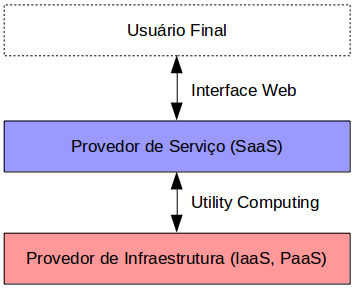
\includegraphics[scale=.6]{imgs/business-model.png}
\caption{Modelo de negócio da computação em nuvem.} 
\label{business-model}
\end{figure}


%%%%%%%%%%%%%%%%%%%%%%%%%%%%%%%%%%%%%
\section{Arquitetura} \label{cloud:arch}
%%%%%%%%%%%%%%%%%%%%%%%%%%%%%%%%%%%%%

Para Zhang et al.~\citeyearpar{stateOfArt:2010} a arquitetura da computação em Nuvem é divida em quatro camadas: a camada de hardware, a camada de infraestrutura, a camada de plataforma e a camada de aplicação, como apresentado na Figura \ref{architecture1}. As camadas são detalhadas abaixo:

\begin{figure}[htbp]
  \centering 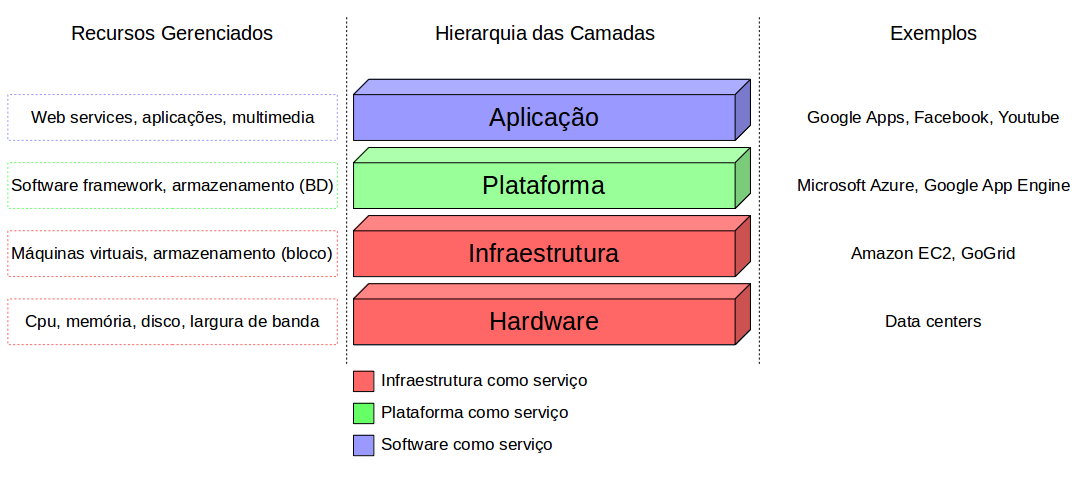
\includegraphics[scale=.4]{imgs/architecture1.png}
\caption{Arquitetura da Computação em Nuvem segundo~\citep{stateOfArt:2010}} 
\label{architecture1}
\end{figure}

\begin{description}

	\item[Camada de Hardware:] essa camada é responsável pela gestão dos recursos físicos, incluindo servidores, roteadores, switches, sistemas de resfriamento e energia. Na prática, a camada de      hardware é tipicamente implementada nos data centers. Um data center normalmente contém milhares de servidores organizados em racks e interconectados através de switches ou roteadores. Problemas típicos na camada de hardware envolvem configuração de hardware, tolerância a falhas, gerenciamento do tráfego, gerenciamento de energia e gerenciamento dos recursos de resfriamento.

	\item[Camada de Infraestrutura:] também conhecida como camada de virtualização, a camada de infraestrutura cria uma pool de armazenamento e recursos computacionais através do particionamento dos recursos físicos utilizando tecnologias de virtualização como  Xen~\cite{Xen:Online}, KVM~\cite{KVM:Online} e VMware~\cite{VMware:Online}. Como as principais características da computação em nuvem, como alocação dinâmica de recursos, só são possíveis por causa das tecnologias de virtualização, a camada de infraestrutura é considerada um componente essencial na arquitetura.

	\item[Camada de Plataforma:] construída sobre a camada de infraestrutura, a camada de plataforma consiste em sistemas operacionais e frameworks. O propósito da camada de plataforma é facilitar o lançamento de aplicações em máquinas virtuais. Por exemplo, o Google App Engine opera na camada de plataforma provendo uma API com suporte para armazenamento e lógica de negócio para aplicações web típicas. 

	\item[Camada de Aplicação:] no nível mais alto da hierarquia, a camada de aplicação consiste nas aplicações da nuvem. Diferentes das aplicações tradicionais, as aplicações da nuvem fazem uso do escalonamento automático disponível na Nuvem para alcançar um melhor desempenho, disponibilidade e baixo custo de operação.

\end{description}

Comparado aos ambientes de hospedagem de serviços tradicionais como servidores dedicados, a arquitetura da nuvem é mais modular. Cada camada é fracamente acoplada, com camadas acima e abaixo, permitindo que cada camada evolua separadamente. Essa modularidade permite que a computação em nuvem dê suporte a uma gama de requerimentos das aplicações enquanto reduz o sobrecusto de manutenção e de administração.

Para Hassan et al.~\citeyearpar{demystifingCloud:2011} a arquitetura também é dividida em quatro camadas com uma hierarquia baseada na abstração, porém a arquitetura é definida diretamente ligada aos modelos de negócio, como pode ser observado na Figura \ref{architecture2}. Nessa definição é adicionando um novo modelo de negócio: dados como serviço, que é descrito como o serviço que oferece base de dados para armazenamento das informações do cliente. 

\begin{figure}[htbp]
  \centering 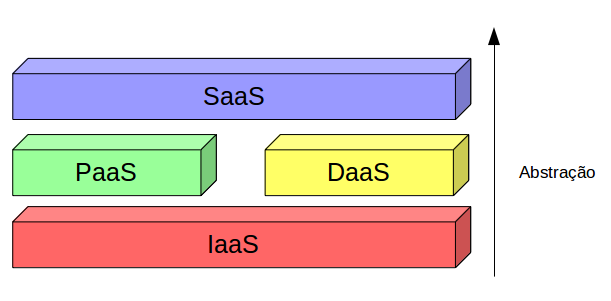
\includegraphics[scale=.6]{imgs/architecture2.png}
\caption{Arquitetura da Computação em Nuvem segundo~\citep{demystifingCloud:2011}} 
\label{architecture2}
\end{figure}

%%%%%%%%%%%%%%%%%%%%%%%%%%%%%%%%%%%%%
\section{Tipos de Nuvem} \label{cloud:types}
%%%%%%%%%%%%%%%%%%%%%%%%%%%%%%%%%%%%%

	Zhang et al.~\citeyearpar{stateOfArt:2010} e Mell et al.~\citeyearpar{NIST:2011} descrevem 4 tipos de nuvem: Nuvem Pública, Nuvem Privada, Nuvem Híbrida e Nuvem Comunitária.

	\begin{description}
	
		\item[Nuvem Pública:] nuvem onde os provedores de serviços oferecem seus recursos ao público geral. Nuvens públicas oferecem vários benefícios aos provedores de serviço: por exemplo, não é necessário para os provedores investimentos inciais em infraestrutura. No entanto, as nuvens públicas oferecem um baixo grau de controle sobre os dados, a rede e as configurações de segurança.  	 
			
		\item[Nuvem Privada:] também conhecida como nuvem interna, as nuvens privadas são para uso exclusivo de uma organização. A nuvem privada pode ser construída e gerenciada pela própria empresa ou por provedores externos. Esse tipo de nuvem oferece um maior controle de desempenho, segurança e confiabilidade. No entanto, as nuvens privadas são criticadas por serem muito similares aos servidores tradicionais.
		
		\item[Nuvem Híbrida:] uma nuvem híbrida é a combinação da nuvem privada e da nuvem pública, na tentativa de minimizar as limitações das duas abordagens. Nesse tipo de nuvem, parte dos serviços de infraestrutura estão na nuvem privada enquanto que as outras partes são executadas em uma nuvem pública. Nuvens híbridas oferecem mais flexibilidade que as nuvens públicas e do que as nuvens privadas. Elas oferecem mais controle sobre dados, rede e segurança do que as nuvens públicas mantendo as facilidades de expansão.
		
		\item[Nuvem Comunitária:] a nuvem comunitária funciona praticamente como uma nuvem privada que pode ser utilizada por duas ou mais organizações. Ela pode ser gerenciada tanto por uma organização, pelas duas organizações, ou por um provedor.
		 	
	\end{description}
	
%%%%%%%%%%%%%%%%%%%%%%%%%%%%%%%%%%%%%
\section{Desafios} \label{cloud:chal}
%%%%%%%%%%%%%%%%%%%%%%%%%%%%%%%%%%%%%

	Apesar da Computação em Nuvem estar amplamente presente na indústria, as pesquisas nessa área ainda estão em fase inicial~\cite{stateOfArt:2010}.  Muitos problemas existentes ainda não foram resolvidos, enquanto novos desafios continuam surgindo das aplicações nas indústrias. Esta seção apresenta um resumo dos principais desafios da Computação em Nuvem. 
	
	\subsection{Provisionamento Automático de Serviço}
	Umas das principais características da Computação em Nuvem é a capacidade de adquirir e liberar recursos sob demanda. O objetivo de um provedor de serviço neste caso é de alocar e desalocar recursos da nuvem a fim de satisfazer os Service Level Objectives (SLOs), enquanto minimiza o custo operacional.  No entanto, não é óbvio como o provedor de serviço alcançará esse objetivo. Em particular, não é fácil de determinar como mapear SLOs tais como requisitos de QoS para requisitos dos recursos de baixo nível como requisitos de CPU e de memória. Além disso, para alcançar alta agilidade para responder as flutuações de demanda, as decisões de provisionamento devem ser feitas em tempo real.
	
	\subsection{Migração de Máquinas Virtuais}
	A virtualização é uma das principais tecnologias utilizadas em infraestruturas em nuvem. Através do uso da virtualização, é possível compartilhar a mesma máquina física com múltiplos sistemas operacionais e/ou aplicações de usuários finais, promovendo o isolamento entre os mesmos. Da mesma forma, o seu uso torna possível realizar balanceamento de carga entre estruturas físicas, através de ações como a migração de máquinas virtuais entre servidores.
	
	A migração de VMs evoluiu das técnicas de migração de processos~\cite{Osman:2002}. Algumas ferramentas já implementam o conceito de live-migration, onde as VMs são movidas em um processo que envolve paradas extremamente curtas que variam de dezenas de milissegundos a um segundo. Clark et al.~\citeyearpar{Clark:2005} mostra que a migração de um SO inteiro e todas suas aplicações como uma unidade permite que muitas das dificuldades encontradas nas abordagens de migração de processos sejam evitadas.
	 
	O maior benefício da migração de VMs é a capacidade de evitar a sobrecarga de pontos específicos da infraestrutura de servidores. No entanto, essa não é uma tarefa simples. Atualmente, a detecção de pontos de sobrecarga e o disparo de uma migração não tem agilidade suficiente para responder às mudanças de carga de trabalho repentinas~\cite{stateOfArt:2010}. Além disso, é necessário transferir o estado dos dados em memória de forma consistente e eficiente, considerando os recursos para as aplicações e para os servidores físicos.
	
	\subsection{Consolidação de Servidores}
	A consolidação de servidores é uma abordagem que tem como objetivo maximizar a utilização de recursos enquanto minimiza o consumo de energia. A técnica de migração de VMs é frequentemente utilizada na consolidação de servidores, onde VMs são movidas de múltiplos servidores subutilizados para um servidor. Dessa forma os servidores restantes são colocados no estado de economia de energia. O problema de consolidar servidores de forma ótima pode ser visto como uma variação do problema bin-packing~\cite{Chekuri:1999}, que é um problema de otimização NP-difícil.
	
	\subsection{Gerenciamento de Energia}
	Atingir uma maior eficiência no consumo de energia também é um dos principais desafios da computação em nuvem. Hamilton et al.~\citeyearpar{Hamilton} estima que o custo de alimentação energética e refrigeração somam 53 por cento dos gastos operacionais dos data centers. Em 2006, os data centers nos Estados Unidos consumiram mais de 1.5 porcento de toda energia gerada naquele ano, e o crescimento dessa porcentagem tem projeção de crescimento de 18 porcento ao ano. Isso leva a uma enorme pressão sobre os provedores de infraestrutura para a redução do consumo energético. O objetivo não é apenas reduzir o gasto energético, mas também se adequar aos regulamentos do governo e as normas ambientais. 
	
	\subsection{Segurança dos Dados}
	A segurança dos dados é outro tópico de pesquisa muito importante na computação em nuvem. Visto que os provedores dos serviços tipicamente não têm acesso aos sistemas de segurança dos data centers, eles dependem do provedor de infraestrutura para garantir a segurança de seus dados. Os provedores de infraestrutura devem garantir:
	\begin{description}
		\item[Confidencialidade] para garantir a segurança de acesso e transferência de dados.
                   
		\item[Auditabilidade] para atestar se as configurações de segurança de uma aplicação foram modificadas ou não.  
	\end{description}	 
	
	Confidencialidade é normalmente alcançada utilizando protocolos de criptografia, enquanto que a auditabilidade é alcançada utilizando técnicas de atestado remoto. Atestados remotos tipicamente necessitam de um trusted platform module (TPM) para gerar um sumário do sistema infalsificável como prova da segurança do sistema. Porém num ambiente como a nuvem onde as VMs podem migrar dinamicamente de um servidor para outro, utilizar atestado remoto não é o suficiente. É necessário que seja criado um mecanismo confiável em cada camada da arquitetura. Inicialmente, para ser confiável, a camada de hardware deve usar um TPM. A camada de infraestrutura, responsável pela migração das VMs, deve utilizar monitores de VMs confiáveis. A migração de VMs só deve ser permitida se tanto o servidor de destino quanto fonte são confiáveis.



\chapter{Plataformas da Nuvem de Código Aberto}

As Plataformas da Nuvem de Código Aberto foram criadas com a intenção de suprir a necessidade de que as soluções IaaS forneçam privacidade e controle sobre os ambientes virtualizados~\cite{Barkat:2015}. Portanto essas plataformas eram usadas principalmente para contruir Nuvens privadas. Atualmente elas são utilizadas para Nuvens públicas, privadas e hibridas. Com o aparecimento de diferentes Plataformas da Nuvem de Código Aberto, mesmo tendo as caracteristicas específicas de cada plataforma, escolher a mais adequada é uma tarefa complicada~\cite{Barkat:2015}.

Muitos trabalhos foram desenvolvidos com objetivos de comparar as diferentes soluções para IaaS. A tabela~\ref{researchesTable} apresenta os trabalhos que comparam as soluções para nuvem, destacando as soluções analisadas, suas limitações e foco.

%%TABELA A FAZERRR
\begin{table}
  \begin{center}
    \caption{Comparação dos estudos sobre as plataformas da Nuvem}\label{researchesTable}
    \begin{tabular}{|p{4cm}|p{6cm}|p{5cm}|}
      \hline
      Estudo & Plataformas Analisadas & Foco/Limitação\\
      \hline
      {\small Voras et. al.~\citeyearpar{Voras:2011}} & {\small Open Nebula, Eucalyptus, Ubuntu Enterprise Cloud, openQRM, Abiquo, Red Hat Cloud Foundation, OpenStack, Nimbus e mOSAIC} & {\small Breve introdução das plataformas, nenhuma comparação fornecida}\\
      \hline
      {\small Zeng et. al.~\citeyearpar{Zeng:2012}} & {\small Amazon EC2, IBM smart cloud, Google App Engine, Windows Azure, Hadoop, Eucalyptus, OpenNebula e Nimbus} & {\small Breve introdução das plataformas, nenhuma comparação fornecida}\\
      \hline
      {\small Endo et. al.~\citeyearpar{Endo:2010}} & {\small XCP, Nimbus, OpenNebula, Eucalyptus, TPlataform, ECP (Enomalys Elastic Computing) e Apaches VCL} & {\small Breve introdução das plataformas e breve comparação fornecida}\\
      \hline
      {\small Amrani et. al.~\citeyearpar{Amrani:2012}} & {\small Eucalyptus, OpenNebula e Nimbus} & {\small Limitado às novas características e à aparência}\\
      \hline
      {\small Von Laszewski et. al.~\citeyearpar{Laszewski:2012}} & {\small Eucalyptus, OpenNebula, Nimbus e OpenStack} & {\small Foco em escalabilidade}\\
      \hline
      {\small Cordeiro et. al.~\citeyearpar{Cordeiro:2010}} & {\small XCP, Eucalyptus e OpenNebula} & {\small Foco na arquitetura das plataformas e na rede}\\
      \hline
      {\small Baset~\citeyearpar{Baset:2012}} & {\small OpenStack e CloudStack} & {\small Detalhes aprofundados apenas para o OpenStack}\\
      \hline
    \end{tabular}
  \end{center}
\end{table}

Alguns trabalhos analizaram algumas soluções mais profundamente considerando um ponto de vista específico. Amrani et. al.~\citeyearpar{Amrani:2012} foca na aparência e nas features, enquanto que Laszewski et. al.~\citeyearpar{Laszewski:2012} foca em comparar a escalabilidade das plataformas e Cordeiro et. al.~\citeyearpar{Cordeiro:2010} nas placement policies, arquitetura das plataformas e na estrutura de rede das plataformas analisadas. Baser~\citeyearpar{Baset:2012} detalha sobre o OpenStack e o CloudStack, porém apenas o OpenStack é analisado profundamente.

Esse capítulo tem como objetivo analisar 5 soluções de código aberto para IaaS: OpenStack, CloudStack, OpenNebula, Eucalyptus e Nimbus e comparar suas características.

%%%%%%%%%%%%%%%%%%%%%%%%%%%%%%%%%%%%%
\section{OpenStack}
%%%%%%%%%%%%%%%%%%%%%%%%%%%%%%%%%%%%%

OpenStack é um software pra Nuvem que oferece a capacidade de controlar uma enorme quantidade de recursos de computação, de rede e de armazenamento. Ele ainda prove ao usuário recursos sob demanda~\cite{OpenStackIntro:Online}. O desenvolvimento do OpenStack começou em 2010, inicialmente sendo desenvolvido pela Rackspace Hosting e pela NASA~\cite{OpenStack:Online} com o objetivo de prover uma solução de código aberto para construção de Nuvens privadas. A missão do OpenStack é permitir que qualquer organização crie e ofereça serviços de Computação em Nuvem. Disponível como uma solução de código aberto, o OpenStack foi construido com 4 princípios em mente:

\begin{description}

	\item[\textit{Open Source}:] todo código é públicado sob a licença Apache 2.0, permitindo a comunidade a utiliza-lo livremente.

	\item[\textit{Open Design}:] a cada 6 meses a comunidade de desenvolvimento realizam um \textit{design summit} para recolher requerimentos e escrever especificações para as próximas versões.

	\item[\textit{Open Development}:] durante toda faze de desenvolvimento de uma nova versão é mantindo públicamente em um repositório o código fonte.

	\item[\textit{Open Community}:] manter as comunidades  de desenvolvimento e de usuários engajadas através de um processo aberto e transparente.   

\end{description}

A primeira versão do OpenStack se chamava Austin e foi lançada em outubro de 2010. Desde então o OpenStack adotou uma politica de realizar 2 lançamentos grandes por ano, totalizando 12 lançamentos até hoje (o próximo será o Mikata, esperado para fevereiro de 2016). O versão Austin continha apenas o componente de armazenamento de objetos (Swift) e o componente de computação (Nova) e apresentava restrições importantes como suporte limitado a objetos de 5GB. O suporte a objetos maiores foi introduzido na segunda versão, chamado Bexar, junto com o serviço de registro de imagem e o serviço de entrega (Glance). Após isso, novos modulos foram introduzidos apenas na quinta versão, chamada de Essex, que introduziu uma interface gráfica para o usuário (Horizon) e um componente de segurança (Keystone). A sexta versão, Folsom, trouxe a rede como um dos projetos principais do OpenStack (antigamente chamado de Quantum, atualmente chamado de Neutron) e um componente de armazenamento de bloco (Cinder). Folsom foi a primeira versão a encorporar os três mais importantes módulos do OpenStack: Swift, Nova e Neutron. Apartir dessa versão os módulos existentes foram fixados e melhorados e alguns serviços compartilhados novos foram adicionados como: serviço de telemetria (Ceilometer) e serviço de orquestração (Heat), foram lançados na oitava versão, Havana. Na nona versão, Icehouse, foi lançado um serviço de banco de dados (Trove). O serviço de processamento de dados (Sahara) foi lançado na décima versão, Juno. Na décima primeira versão, Kilo, foi introduzido o serviço de \textit{bare metal} (Ironic). Na mais nova versão, Liberty, foi lançado um serviço de busca (Searchlight).

\subsection{Arquitetura Base}

Como em qualquer outro plataforma para Nuvem, a infraestrutura por baixo do OpenStack é formada por hardware padrão, que pode conter qualquer peça de dispositivos físicos como servidores, discos ou dispositivos de rede. No intuito de prover serviços na nuvem, o OpenStack desenvolveu camadas de virtualização, promovendo uma abstração da infraestrutura física para o usuário final. Essas camadas de virtualização são desenvolvidas numa arquitetura multicomponente.

A arquitetura do OpenStack consiste em 3 componentes principais: computação (Nova), rede (Neutron) e armazenamento (Swift). Além desses 3 componentes, o OpenStack vem desenvolvendo muitos outros serviços, projetados para trabalharem juntos para prover uma solução IaaS completa. A integração desses serviços é facilitada através de APIs (\textit{application programming interfaces}) que são fornecidas por cada serviço~\cite{OpenStack:Online}.

\subsubsection{Computação (Nova)}

O componente de computação, de codinome Nova e escrito em Python, é responsável por gerenciar grandes redes de VMs e eventualmente por escalonar as VMs entre as máquinas físicas disponíveis~\cite{OpenStack:Online}. O Nova é uma aplicação distribuída que consiste em 6 componentes: Nova-api, Message Queue, Nova-Compute, Nova-Network, Nova-Volume e Nova-Scheduler. O Nova suporta o ciclo-de-vida completo de uma instância na Nuvem, desde a requisição para inicializar uma VM até seu término. Os seis componentes são detalhados abaixo:

\begin{description}

	\item[Nova-api:] aceita e responde as chamadas do usuário de computação do usuário final pela API. Além de prover sua própria API, o Nova-api é compatível com a API da Amazon EC2, oferecendo o potencial de integração com os serviços de Nuvem da Amazon. Esse componente lida com a organização das atividades como: executar uma instância e aplicação de políticas de execução.

	\item[Nova-compute:] é responsável por criar e terminar as instâncias de VM através das APIs do hypervisor. OpenStack suporta vários hypervisors capacidade de aceitar outros hypervisor através de sua biblioteca padrão.

	\item[Nova-volume:] gerencia a criação, a ligação e a desligação de volumes persistentes para instâncias de computação. Existem dois tipos de armazenamentos suportados por uma VM: (1) Armazenamento Efêmero, que é associada com uma unica instância. Um bloco de armazenamento efêmero é conectado ao ciclo-de-vida de uma instancia, quando essa instância terminar os dados são deletados; (2) Armazenamento de Volume: é persistente e independente de qualquer instância particular. 

	\item[Nova-network:] responsável por todas tarefas relacionadas a rede. Tarefas como trocar a as regras da tabela de ips ou setar as interdaces de \textit{bridge}.

	\item[Nova-schedule:] responsável pelo escalonamento de VMs entre as máquinas físicas. Enquanto os algoritmos de escalonamento podem ser definidos pelo usuário, o Nova-schedule suporta por padrão 3 algoritmos: (1) Simple: tenta encontrar o \textit{host} mais livre, (2) Chance: escolhe um \textit{host} aleatório disponível da tabela de serviço, (3) Zone: escolhe um \textit{host} aleatório em uma zona disponível. Ao permitir que os usuários definam seus próprios algoritmos de balanceamento faz desse componente muito importante para a construção de um sistema tolerante a falhas e com balanceamento de carga.

	\item[Queue:] é uma central para a passagem de mensagens entre os componentes. É normalmente implementado com RabbitMQ, mas suporta outros tipos de fila de mensagens.

	\item[Database:] armazena a maior parte do estado de execução e do estado de construção da infraestrutura da Nuvem. Por exemplo, o Database fornece informação das instancias que estão disponíveis para uso e em uso, redes disponíveis e informação de armazenamento. O Nova, teoricamente, suporta qualquer banco de dados baseado em SQL, mas os bancos de dados mais usados são sqlite3, MySQL e PostgresSQL.

\end{description}

Todos os componentes da arquitetura do OpenStack seguem uma política \textit{shared-nothing} baseada em mensagens. \textit{Shared-nothing} significa que cada componente de cada grupo de componentes pode ser instalado em qualquer servidor, de maneira distribuida, enquanto que ser baseado em mensagens garente que a comunicação entre todos os componentes seja realizada através de uma fila de mensagens. 

\subsubsection{Rede (Neutron)}

O componente de rede de qualquer plataforma na Nuvem tem funções importantes: (1) oferecer acessibilidade aos recursos e serviços, (2) prover a ligação dos endereços entre diferentes serviços e (3) configurar automaticamente a rede.

A arquitetura do Neutron consiste em quatro redes físicas distintas:

\begin{description}

	\item[Rede de Gerenciamento:] usada para comunicação interna entre os componentes do OpenStack. 

	\item[Rede de Dados:] usada para comunicação com VMS relacionada a dados na Nuvem.

	\item[Rede Externa:] usada para prover acesso a Internet à VMs.

	\item[Rede da API:] expõe todas APIs do OpenStack.

\end{description}


\subsubsection{Armazenamento}

O componente de armazenamento tem como finalidade gerenciar os recursos armazenados. OpenStack tem suporte tanto para Armazenamento de Objetos quanto para Armazenamento de Bloco.

O Swift, componente responsável pelo armazenamento de objetos, provê uma API de acesso a plataforma que pode ser integrada diretamente com aplicações ou utilizada para \textit{backup}, arquivamento e retenção de dados~\cite{OpenStack:Online}. No armazenamento de objetos os dados são salvos em multiplos dispositivos de hardware, o OpenStack fica responsável por garantir a replicação dos dados e a integridade entre os \textit{clusters}. 

O armazenamento de bloco é responsabilidade do componente chamado de Cinder. Por gerenciar os recursos de armazenamento em blocos, o armazenamento em bloco é apropriado para cenários que precisam de desempenho como armazenamento de banco de dados.

\subsubsection{Interface Gráfica (Horizon)}

O OpenStack fornece uma interface gráfica tanto para usuários quanto para administradores, capaz de controlar os recursos de computação, armazenamento e rede. Através do Horizon os administradores podem gerenciar os usuários e os limites de acesso para cada usuário.

\subsubsection{Serviços Compartilhados}

Os Serviços Compartilhados do OpenStack é um conjunto de serviços presentes nos 3 principais módulos do OpenStack com o objetivo de facilitar as operações de gerenciamento da Nuvem. Serviços como de identidade, de imagem, de telemetria, de orquestração e de banco de dados~\cite{OpenStack:Online}:

\begin{description}

	\item[Serviço de identidade (Keystone):] é o serviço de sergurança, usado para proteger o acesso e uso dos recursos.

	\item[Serviço de Imagem (Glance):] é o repositório para discos virtuais e das imagens usadas pelas VMs.

	\item[Serviço de Telemetria (Ceilometer):] capaz de analizar a utilização dos recursos e a performace dos serviços do OpenStack.

	\item[Serviço de Orquestração (Heat):] permite que os desenvolvedores de aplicações descrevam e automatizem o lançamento de infraestruturas na Nuvem.

	\item[Serviço de Banco de Dados (Trove):] permite que usuários utilizem as características dos banco de dados relacionais. Usuários e administradores de banco de dados podem criar e gerenciar multiplas instancias de banco de dados.

\end{description}

\subsubsection{Propriedades}

O OpenStack é construido seguindo uma filosofia livre: no sentido de evitar estar diretamente ligado a tecnologias específicas e fornecer ao usuário a liberdade de escolher as tecnologias que melhor se encaixam as suas necessidades~\cite{OpenStack:Online}. Abaixo é feita uma analise sobre as principais propriedades do OpenStack.

\begin{description}

	\item[\textit{Live migration}:] O OpenStack suporta dois tipos de \textit{live migration}: baseada em armazenamento compartilhado e \textit{live migration} por bloco.

	\item[Balanceamento de carga:] O OpenStack suporta balanceamento de carga em diferentes niveis. A propriedade de \textit{live migration} permitiu que os administradores do sistema distribuam as cargas de trabalho entre os servidores físicos através do ajuste da localização da VM. Além disso, é possível controlar as cargas de trabalho a nível de VM. O OpenStack tem um projeto em desenvolvimento chamado Load Balancing as a Service (LBaaS) que tem objetivo fornecer um serviço de balanceamento de carga para usuário final.

	\item[Tolerância a falhas:] a tolerância  falhas também pode ser feita em diferentes niveis, dependendo da maneira que o IaaS foi configurado. No nível de VM, com objetivo de prever falhas, o usuário pode desenvolver algoritmos de escalonamento (além dos três já existentes). A nível de armazenamento e de banco de dados, a tolerância a falhas é alcançada através da replicação e sincronização garantindo que a falha em um dispositivo não pare todo sistema.

	\item[Disponibilidade:] 

	\item[Segurança:] OpenStack tem um serviço separado (Keystone) que fornece um gerenciamento central de autenticação para os usuários e o sistema operacional da nuvem.

	\item[Compatibilidade:] o OpenStack é compatível com o Amazon EC2 e Amazon S3. As aplicações de cliente feitas para a Amazon Web Service podem ser usadas com OpenStack apartir de um esforço mínimo~\cite{OpenStack:Online}. O OpenStack tem suporte para vários \textit{hypervisors}: Xen, KVM, HyperV, VMWare, etc.

\end{description}


%%%%%%%%%%%%%%%%%%%%%%%%%%%%%%%%%%%%%
\section{CloudStack}
%%%%%%%%%%%%%%%%%%%%%%%%%%%%%%%%%%%%%

%%%%%%%%%%%%%%%%%%%%%%%%%%%%%%%%%%%%%
\section{Eucalyptus}
%%%%%%%%%%%%%%%%%%%%%%%%%%%%%%%%%%%%%

%%%%%%%%%%%%%%%%%%%%%%%%%%%%%%%%%%%%%
\section{OpenNebula}
%%%%%%%%%%%%%%%%%%%%%%%%%%%%%%%%%%%%%

%%%%%%%%%%%%%%%%%%%%%%%%%%%%%%%%%%%%%
\section{Nimbus}
%%%%%%%%%%%%%%%%%%%%%%%%%%%%%%%%%%%%%





\chapter{Conclusão}

% Bibliografia
% http://liinwww.ira.uka.de/bibliography/index.html
% um site que cataloga no formato bibtex a bibliografia em computacao
%\bibliography{nomedoarquivo.bib} (sem extensao)
%\bibliographystyle{formato.bst} (sem extensao)

\bibliography{bibliografia}
\bibliographystyle{abnt}

% Anexos (Opcional)
\annex 

\end{document}

